\documentclass{ucph-handout}
\usepackage[danish]{babel}

\newcounter{handout}
\stepcounter{handout}
\newcommand{\Ark}{Arbejdsark \arabic{handout}: }
\renewcommand{\Title}{\Ark LED-strip}%
\renewcommand{\Author}{Martin Dybdal}
\renewcommand{\AuthorEmail}{dybber@di.ku.dk}

\begin{document}
\begin{exercisebox}[adjusted title=Tilslut LED-strip]
Tilslut jeres LED-strip som vist på billedet. Brug et mellemled (3 x jumper kabel).
\begin{center}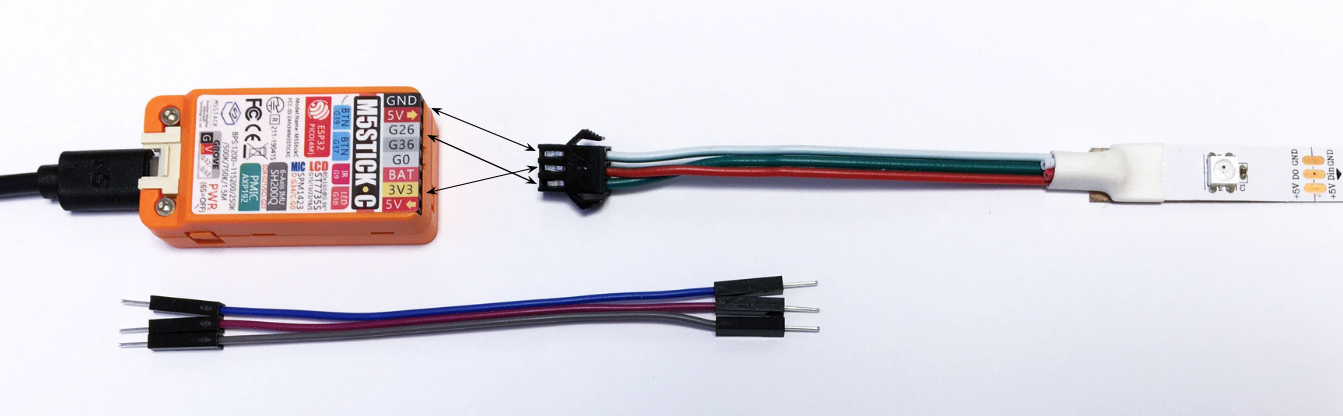
\includegraphics[width=1.0\textwidth]{illustrationer/m5stickc_ledstrip_connection3}
\end{center}

Forbindelserne er:
\begin{center}
\begin{tabular}{llll}
  \textbf{Type} & \textbf{Microcontroller} & \textbf{LED-strip ledning} \\
  \hline
 Jord & GND & Hvid \\
  Strøm (3,3 volt) & 3V3 & Rød \\
 Data / kontrolsignal & G26 & Grøn
\end{tabular}
\end{center}
\end{exercisebox}

\begin{exercisebox}[adjusted title=Første MicroPython program]
Åbn Mu-editoren. Opret en fil ``intro.py'' med dette indhold:
\begin{python}
import machine
import tinkerlib

# 30 LED'er tilsluttet pin 26
ledstrip = tinkerlib.LEDStrip(machine.Pin(26), 30)

# Indstil LED'ernes farver
ledstrip[0] = (255, 0, 0)
ledstrip[9] = (0, 0, 255)

# Opdater LED'erne ved at kalde ledstrip.write()
ledstrip.write()
\end{python}

\tcbsubtitle{Afprøv programmet}
\begin{itemize}
\item Tryk på 
\includegraphics[width=10mm]{illustrationer/run-button}-knappen i Mu for at køre programmet på Microcontrolleren.
\item Tjek, at den første diode lyser rødt (diode 0) og den tiende lyser blåt (diode 9).
\end{itemize}

\tcbsubtitle{Øvelse}
\begin{itemize}
\item Udvid programmet, så hver anden diode farves rød og hver anden farves blå for de første 10 dioder.
\end{itemize}
\end{exercisebox}
\newpage
%\vspace{-30mm}
\begin{exercisebox}[adjusted title=Navngivning]
  \vspace{-1mm}
  Vi kan gøre programmet nemmere at læse, ved at give navne til
  farvekoderne. Navngiv farverne i \ttpy{intro.py}:
 \vspace{-1mm}
\begin{python}
# Opret nye navne 'red' og 'blue'
red = (255, 0, 0)
blue = (0, 0, 255)

# Brug navne i koden - det gør det nemt at læse og ændre
ledstrip[0] = red
ledstrip[1] = blue
ledstrip[2] = red
...
ledstrip[9] = blue
ledstrip.write()
\end{python}
\vspace{-4mm}
\end{exercisebox}

\begin{exercisebox}[adjusted title=Animationer]
\vspace{-1mm}
For at lave animationer skal vi bruge funktionen \ttpy{sleep_ms} fra
biblioteket \ttpy{time}.
\vspace{-1mm}
\begin{python}
import machine
import tinkerlib
import time
ledstrip = tinkerlib.LEDStrip(machine.Pin(26), 30)

# Tænd den første diode
ledstrip[0] = (255, 0, 0)
ledstrip.write()
time.sleep_ms(200) # Vent 200 millisekunder

# Tænd den næste diode
ledstrip[1] = (0, 0, 255)
ledstrip.write()
time.sleep_ms(200) # Vent 200 millisekunder

# Fortsæt selv ...
\end{python}
\vspace{-3mm}
\tcbsubtitle{Øvelser}
\vspace{-4mm}
\begin{itemize}
\item Fortsæt mønsteret for de første 10 LED'er.
\item Lav en variabel til at styre hastigheden (i stedet for at gentage "`200"')
\item En LED slukkes ved at sætte den til (0, 0, 0). Sluk den forrige
  LED i hvert trin, så der kun er en LED tændt ad gangen.
\end{itemize}
  \vspace{-5mm}
\end{exercisebox}

\begin{exercisebox}[adjusted title=Flere farver]
  \vspace{-2mm}
  Her er nogle flere farver I kan bruge. Lav fx en regnbue, en istap, en
  animation af ild, eller noget andet i selv finder på.
  \hfill \\
  \begin{minipage}{0.45\linewidth}
    \begin{tabular}{ll}
    \textbf{Rød} & \lstinline[style=mypython]$(255, 0, 0)$ \\
    \textbf{Grøn} & \lstinline[style=mypython]$(0, 255, 0)$ \\
    \textbf{Blå} & \lstinline[style=mypython]$(0, 0, 255)$ \\
%    \textbf{Hvid} & \lstinline[style=mypython]$(255, 255, 255)$ \\
    \end{tabular}
  \end{minipage}
  \begin{minipage}{0.45\linewidth}
    \begin{tabular}{ll}
%    \textbf{Slukket} & \lstinline[style=mypython]$(0, 0, 0)$ \\
    \textbf{Gul} & \lstinline[style=mypython]$(255, 255, 0)$ \\
   \textbf{Lilla} & \lstinline[style=mypython]$(127, 0, 255)$ \\
    \textbf{Tyrkis} & \lstinline[style=mypython]$(0, 255, 255)$ \\
    \end{tabular}
  \end{minipage}

  \tcbsubtitle{Flere muligheder}
  I kan også gøre brug af funktionerne
  \ttpy{ledstrip.fill(farve)}, \ttpy{ledstrip.clear()} eller
  \ttpy{ledstrip.fillN(farve, antal)}, der hhv. tænder alle, slukker
  alle eller tænder et specifikt antal LED'er.
\end{exercisebox}

% \newpage
% TODO: Ekstra ark om LEDStrip.fill(), LEDStrip.fillN(), LEDStrip.clear()
% evt. en opgave med en løkke

\newpage
\stepcounter{handout}
\renewcommand{\Title}{\Ark Fugtighedssensor}
\begin{exercisebox}[adjusted title=Tilslut fugtighedssensor]
  Fugtighedssensoren, tilsluttes via et specielt stik, ved siden af
  USB-C stikket. Farverne på de fire ledninger har betydning, se tabellen
  nedenfor.

\begin{center}
\begin{minipage}{0.85\linewidth}
\begin{tabular}{llll}
  \textbf{Type} & \textbf{Ledningsfarve} & \textbf{Fugtighedssensor ben} \\
  \hline
 Jord & Sort & - \\
 Strøm (3,3 volt) & Rød & + \\
 Data / kontrolsignal & Gul & out
\end{tabular}
\end{minipage}
\begin{minipage}{0.1\linewidth}
  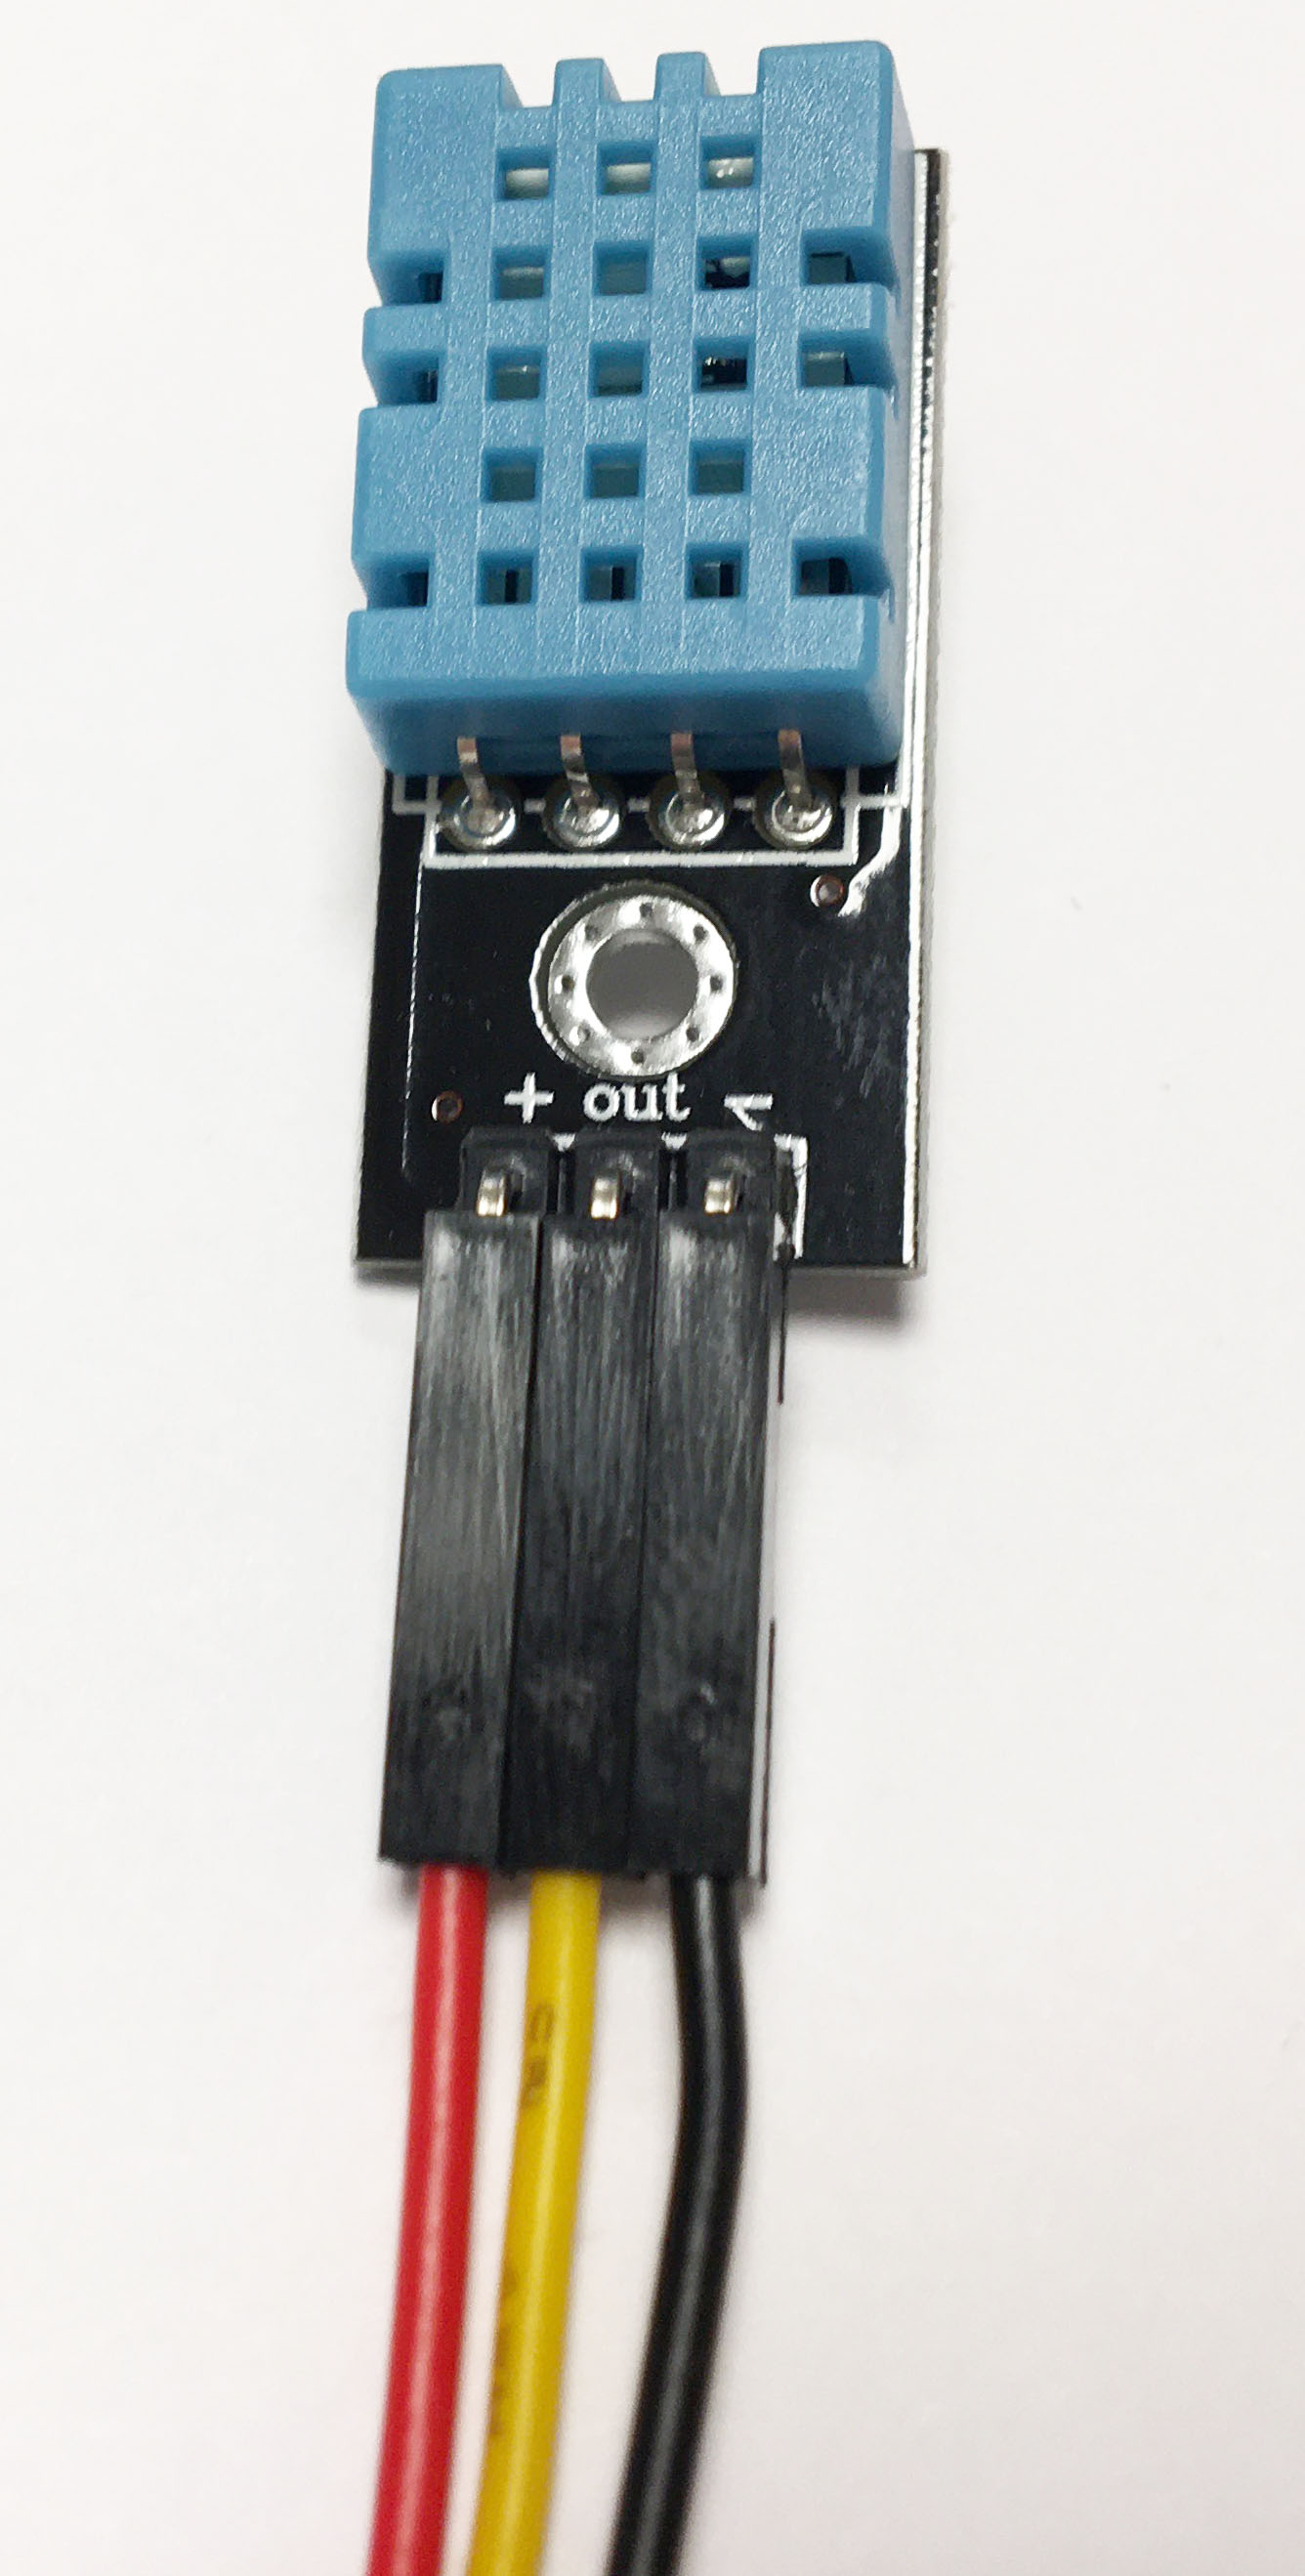
\includegraphics[width=\textwidth]{illustrationer/dht11}
\end{minipage}
\end{center}

\textbf{Vigtigt:} Den må ikke sættes forkert på, tjek evt. farverne en
ekstra gang. (Den hvide ledning bruges ikke og kan evt. klippes af.)
\end{exercisebox}

\begin{exercisebox}[adjusted title=Måling]
  Opret en ny fil i Mu-editoren og gem den som "`\ttpy{measure.py}"'.
  Indtast følgende program for at lave en måling med sensoren:

\begin{python}
import machine
import dht

# Fugtighedssensor tilsluttet via pin 33 (gul ledning)
sensor = dht.DHT11(machine.Pin(33))

sensor.measure()                  # 1) Foretag måling
luftfugtighed = sensor.humidity() # 2) Gem luftfugtighed i variabel
print(luftfugtighed)              # 3) Vis den aflæste værdi
\end{python}

Afprøv programmet (tryk på

\includegraphics[width=5mm]{illustrationer/run-button}). Der bør blive
vist et tal mellem 0 og 100 i konsollen (formentlig omkring
40-55). Det er luftfugtigheden i procent.

\tcbsubtitle{Fejlsøgning}
Hvis I får fejlmeddelelsen \ttpy{ETIMEDOUT}, kan det være tegn på tre forskellige ting:
\begin{itemize}
\item Kablerne er sat forkert i.
\item Stikket er ikke helt trykket i bund. Det skal sige klik når stikket sættes i microcontrolleren.
\item Sensoren er langsom, og I har kørt programmet for mange gange hurtigt efter hinanden.
\end{itemize}
\end{exercisebox}
\newpage
\begin{exercisebox}[adjusted title=Gentag måling]
Vi skal nu ændre programmet, så det bliver ved med at aflæse værdierne. Ændr
programmet til at bruge en "`\ttpy{while True}"', som nedenfor, det
gentager programmet igen og igen. Det er vigtigt at linjerne under
"`while True:"' bliver rykket ind som vist.\\
\vspace{-2mm}

Hold en pause (\ttpy{time.sleep_ms}) mellem hver måling, sensoren er lidt langsom.

\begin{python}
import machine
import dht
import time

# Fugtighedssensor tilsluttet via pin 33 (gul ledning)
sensor = dht.DHT11(machine.Pin(33))

while True:
    sensor.measure()                  # 1) Foretag måling
    luftfugtighed = sensor.humidity() # 2) Gem luftfugtighed i variabel
    print(luftfugtighed)              # 3) Vis den aflæste værdi
    time.sleep_ms(1000)               # 4) Vent 1 sekund
\end{python}

Afprøv programmet (tryk på 
\includegraphics[width=5mm]{illustrationer/run-button})
\end{exercisebox}


\begin{exercisebox}[adjusted title=Fugtighed og LED-strip]

Tilføj i starten af filen:
\begin{python}
import tinkerlib
ledstrip = tinkerlib.LEDStrip(machine.Pin(26), 30)
red = (100, 0, 0)
green = (0, 100, 0)
\end{python}

Tilføj inde i "`\ttpy{while True:}"' konstruktionen (husk fire mellemrum før hver linje):
\begin{python}
color = green
if luftfugtighed > 80:
    color = red   # Udføres kun når luftfugtigheden er > 80%

# Tænd 8 LED'er i den valgte farve
ledstrip.fillN(color, 8)
\end{python}

Afprøv programmet (tryk på 
\includegraphics[width=5mm]{illustrationer/run-button})

\tcbsubtitle{Opgaver}

\begin{itemize}
\item Ændr ottetallet til beregningen \ttpy{luftfugtighed*3/10}, hvad sker der?
% \item Ændr programmet, så det ikke altid tænder 8 LED'er, men tænder
%   et antal proportionelt med luftfugtighed (alle LED'er ved 100\% luftfugtighed,
%   ingen ved 0\%)

%   Hint: I skal altså lave en beregning, der omregner et tal mellem
%   0-100 om til et tal mellem 0-30. Prøv evt. på papir først.
\end{itemize}
\end{exercisebox}

\newpage
\stepcounter{handout}
\renewcommand{\Title}{\Ark Tidstagning}
\begin{exercisebox}[adjusted title=Tilstande]
  For at kunne tage tid på længden af et brusebad, skal vi først holde
  øje med tilstanden, som skifter mellem "`INAKTIV"' og "`BAD"', afhængig af luftfugtigheden:

 \quad\quad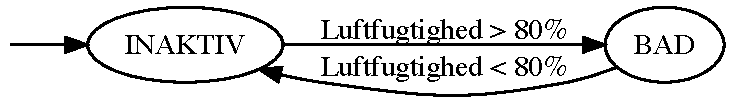
\includegraphics[width=0.55\textwidth]{graphviz/basic.pdf}
  
Tilføj først en ny variabel ovenover "`\ttpy{while}"'
\begin{python}
tilstand = "INAKTIV"

while True:
    # ... samme som før ...
\end{python}

Erstat dernæst "`if-else"' blokken fra før, med følgende der ikke ændrer på LED-strippen, men bare skifter tilstand:
\begin{python}
if luftfugtighed > 80 and tilstand == "INAKTIV":
    tilstand = "BAD"

if luftfugtighed <= 80 and tilstand == "BAD":
    tilstand = "INAKTIV"
\end{python}

\tcbsubtitle{Opgave}
\begin{itemize}
\item Brug \ttpy{print()} til at følge med i om tilstanden ændrer sig, som den skal
\end{itemize}
\end{exercisebox}
\begin{exercisebox}[adjusted title=Tidtagning og nedtælling]
  Vi skal udvide med endnu en tilstand, så vi kan lave en alarm der går af efter 3 minutter.

  \quad\quad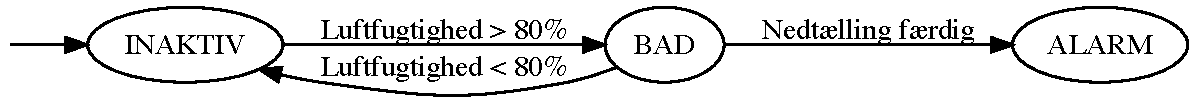
\includegraphics[width=0.8\textwidth]{graphviz/alarm.pdf}  

  % Hver gang alle linjerne i "`\ttpy{while}"' er blevet kørt, går der et
  % sekund pga. vores \ttpy{time.sleep_ms(1000)}. Det skal vi bruge til at
  % tage tid på et brusebad.

  
  For at tælle hvor lang tid der er gået, skal vi bruge en ny variabel
  til at holde styr på tiden med.

Tilføj en variabel \ttpy{timer} ovenover "`\ttpy{while}"':
\begin{python}
timer = 0
\end{python}

Inde i \ttpy{while}-løkken begynder vi så at tælle op. Hver gang hele
\ttpy{while}-løkken er blevet kørt er der gået cirka et sekund,
pga. vores \ttpy{time.sleep_ms{1000}.
\begin{python}
if tilstand == "BAD":
    timer = timer + 1
\end{python}

For at skifte over til alarm tilstanden, skal vi nu bare tilføje endnu en \ttpy{if}:
\begin{python}
if timer > 180 and tilstand == "BAD":
    tilstand = "ALARM"
\end{python}

\tcbsubtitle{Prøv det af}
\begin{itemize}
\item Hvornår skal den skifte tilbage fra \ttpy{"ALARM"}?
\item Husk at sætte timeren tilbage til 0 på et passende sted
\end{itemize}
\end{exercisebox}

\newpage

\begin{exercisebox}[adjusted title=Alarm på LED-strip]
\begin{itemize}
\item Brug print til at følge med i værdien af timeren
\item Gør så LED-strippen viser hvor mange sekunder der er gået
\item Gør så LED-strippen viser hvor mange minutter der er gået
\item Gør så LED-strippen tæller ned fra 5, når et bad starter (spørg
  evt. om et hint)
\end{itemize}
\end{exercisebox}

\begin{exercisebox}[adjusted title=Brug af højtaler]
\begin{minipage}{0.60\linewidth}
Erstat LED-strippen med højtaler og lav en ny fil
\ttpy{speaker_demo.py}, hvor I indtaster:
\begin{python}
import hat
speaker = hat.get(hat.SPEAKER)

speaker.tone(1800, 200)
\end{python}

Det første tal er frekvensen, det andet tal længden af tonen i millisekunder.\\

Man kan desværre ikke have LED-strip og højtaler tilsluttet samtidig.
\end{minipage}
\begin{minipage}{0.30\linewidth}
      \quad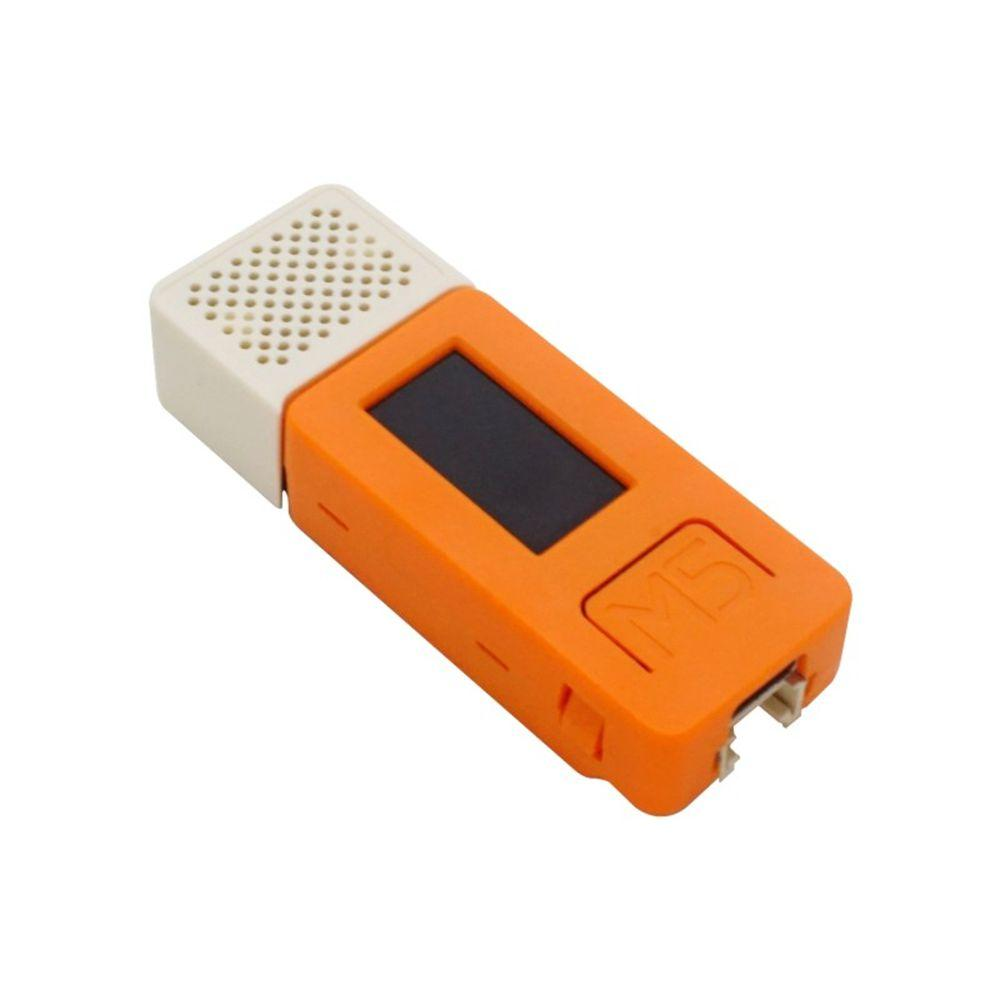
\includegraphics[width=4cm]{illustrationer/m5stickc_speaker}
\end{minipage}
    


\tcbsubtitle{Alarm}
\begin{itemize}
\item Gå tilbage til jeres \ttpy{measure.py}-program, og indsæt kode
  så højtaleren lyder, når tilstanden er \ttpy{"ALARM"}.
\end{itemize}
\end{exercisebox}



\newpage

\stepcounter{handout}
\renewcommand{\Title}{\Ark Få måleren online}
\begin{exercisebox}[adjusted title=Oprettelse på Adafruit]
  \begin{minipage}{0.7\linewidth}
    Åbn hjemmesiden \url{io.adafruit.com}, og opret en bruger ved at trykke på:\\
    
    \quad
\includegraphics[width=2cm]{illustrationer/adafruit_createaccount1}

  \vspace{3mm}
  Udfyld navn, email, brugernavn og password og tryk på "`Create
  account"'.

%  \todo{mail confirm?}
 % \vspace{1cm}
\end{minipage}
\begin{minipage}{0.29\linewidth}
  \begin{center}
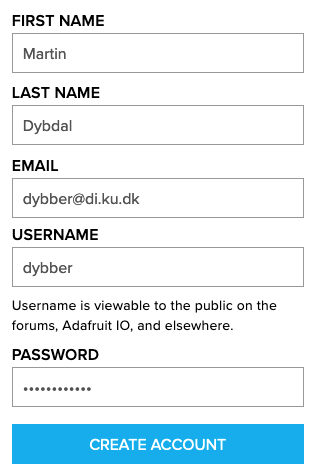
\includegraphics[width=0.7\textwidth]{illustrationer/adafruit_createaccount2}
\end{center}
\end{minipage}

\tcbsubtitle{Opret feed} Gå tilbage til \url{io.adafruit.com}. Vi skal
oprette et \textit{feed} vi kan sende vores luftfugtigheds-data til.

\begin{itemize}
\item Tryk på følgende fire knapper i rækkefølge:

\hspace{1cm}

\includegraphics[width=0.3\textwidth]{illustrationer/adafruit_create_feed1}
\quad
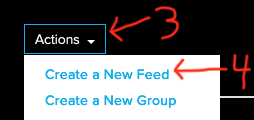
\includegraphics[width=0.3\textwidth]{illustrationer/adafruit_create_feed2}

\item Indtast et navn, fx \textit{humidity} og tryk "`Create"'.
\end{itemize}
% \begin{itemize}
% \item Tryk på 
\includegraphics[width=2cm]{illustrationer/adafruit_feeds_button} øverst
% \item Tryk på "`Create New Feed"':
%   \quad  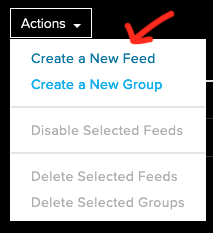
\includegraphics[width=0.3\textwidth]{illustrationer/adafruit_create_feed}
% \end{itemize}

\end{exercisebox}

\begin{exercisebox}[adjusted title=Forbind til WiFi fra microcontroller]
\vspace{-2mm}
Opret en ny fil med følgende indhold og gem som ``\ttpy{adafruit_send.py}'':
\begin{python}
import time
import wifi
import requests
import json

wifi.connect("DIKU1", "PeterNaur")
\end{python}

\noindent
Når I kører filen, burde den skrive følgende (og et par andre
linjer):
\begin{lstlisting}
  Connecting to WiFi network...
  Successfully connected to "DIKU1".
\end{lstlisting}
%\vspace{-4mm}
% \noindent
% Hvis I kører den flere gange skriver den:
% \begin{lstlisting}
% Already connected.
% \end{lstlisting}
\tcbsubtitle{Indtast brugernavn og AIO key} Vi skal bruge jeres
brugernavn og en speciel 'nøgle' for at logge på
\ttpy{io.adafruit.com} fra vores program.

Opret to variabler \ttpy{username} og \ttpy{AIO_KEY}, ved at tilføje følgende:
\begin{python}
  username = "JERES BRUGERNAVN"
  AIO_KEY = "JERES NØGLE"
\end{python}

I finder jeres \textit{AIO Key} ved at trykke på

\includegraphics[width=15mm]{illustrationer/adafruit_aiokey_button}
inde på Adafruit-hjemmesiden. Kopier indholdet af feltet "`Active
Key"'. Der kan fx stå \ttpy{"aio_6f1752f7441f8b01fbd54b949e3b"}. Det
sætter I ind i stedet for \ttpy{"JERES NØGLE"}.
\end{exercisebox}


\begin{exercisebox}[adjusted title=Send data til Adafruit IO]
Næste trin er at få sendt noget data afsted. Til det skal I bruge følgende funktion:
\begin{python}
def send_to_feed(feed, value):
    url = "https://io.adafruit.com/api/v2/"
    url = url + username + "/feeds/" + feed + "/data/"
    headers = {'X-AIO-Key': AIO_KEY}
    data = { "value" : value }
    r = requests.post(url, headers=headers, json=data)
    r.close()
\end{python}
(Kan kopieres fra dette link: \url{kortlink.dk/24mhr})

\vspace{2mm}
For at sende en værdi, fx tallet 17, skriver I:

\begin{python}
send_to_feed("NAVNET PÅ JERES FEED", 17)
\end{python}

I skal bruge navnet på jeres feed, som I oprettede tidligere. Hvis det
ikke virker, så prøv følgende:
\vspace{-1mm}
\begin{itemize}
 \item Find i stedet jeres \textit{Feed key} ved at trykke på:

  \quad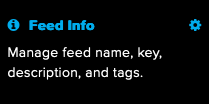
\includegraphics[width=3cm]{illustrationer/adafruit_feedinfo}.
  
  Hvis I ikke kan finde det, skal I måske først åbne "`hamburger"'-menuen: 
\includegraphics[width=5mm]{illustrationer/adafruit_hamburger}
\end{itemize}

\tcbsubtitle{Tjek at det virker}

\begin{itemize}
\item Åbn \ttpy{io.adafruit.com} og klik videre til jeres feed. ("Feeds" -> "Humidity", fx)
\item Tjek at grafen viser tallet 17
  \vspace{-1mm}
\end{itemize}
\end{exercisebox}

\begin{exercisebox}[adjusted title=Send luftfugtighedsdata]
  Nu er det jeres opgave at kombinere de to dele, så data'en I aflæser
  fra jeres fugtighedssensorer, bliver sendt til jeres feed på
  Adafruit.

  Kopier de relevante dele af \ttpy{adafruit_send.py} over i \ttpy{measure.py}
  \begin{itemize}
  \item Import af modulerne \ttpy{wifi}, \ttpy{requests}, \ttpy{json}
  \item Kode der forbinder til WiFi
  \item Definition af \ttpy{username} og \ttpy{AIO_KEY}
  \item Funktionen \ttpy{send_to_feed}
    \vspace{-1mm}
  \end{itemize}
\end{exercisebox}

\begin{exercisebox}[adjusted title=Overfør program til microcontroller]
  Programmet kører kun sålænge microcontrolleren sidder i computeren.

  For at overføre programmet skal I omdøbe det til "`main.py"', og
  bruge "`Files"' menuen i Mu, hvor I skal trække "`main.py"' fra HØJRE side til
  venstre side.

  Genstart microcontrolleren ved at holde knappen på siden,
  nærmest USB-porten inde i 6 sekunder.
\end{exercisebox}


% \stepcounter{handout}
% \renewcommand{\Title}{\Ark Hent data på sekundær microcontroller}
% \begin{exercisebox}[adjusted title=Hent data fra Adafruit IO]
%   Vi skal nu have gang i jeres anden microcontroller, og få den til at
%   hente data om luftfugtighed ned.
  
% Til det skal I bruge funktionen \ttpy{get_data}:
% \begin{python}
% def get_data(feed):
%     url = "https://io.adafruit.com/api/v2/"
%     url = url + username + "/feeds/" + feed + "/data/last?include=value"
%     headers = {'X-AIO-Key': AIO_KEY}
%     r = requests.get(url, headers=headers)
%     data = r.json()
%     r.close()
%     if data:
%         return data["value"]
% \end{python}
% (Kan kopieres fra dette link: \url{kortlink.dk/24mm7})

% \vspace{2mm}
% For at hente seneste værdi, skriver I

% \begin{python}
% a = get_data("NAVNET PÅ JERES FEED")
% \end{python}


% \end{exercisebox}

\end{document}
